%!TEX root = /Users/dylanmorano/Documents/School/Junior/OCE-408/Term Project/git/408term/latex master/modulator.tex
\section{Statement of Problem}

The purpose of this assignment was to investigate the natural forces contributing to littoral transport and beach erosion for re-nourishment purposes. Using 20 years of hind-cast wave height data, 20 and 50 year return period extremes for three dominant wave directions were to be determined. The wave height extrema were also to be determined and fitted with a Gumbel probability distribution function. The results were to be plotted and tabulated.

\section{Hypotheses and Theories}

The Wave Information Studies (WIS) program is an Army Corps of Engineers project which consistently monitors hours, long term wave climatologies along all US coastlines. Wave predictions can be made based off this hind cast data in order to determine future wave characteristics and their effects on the coastline. For this study, weather station 63079 from the WIS program was selected for its close proximity to the Narragansett Town Beach in order to conduct the investigations. A map containing the location of weather station 63079 (outlined in red) can be seen below in Figure 2.1

\begin{figure}[H]
	\centering
	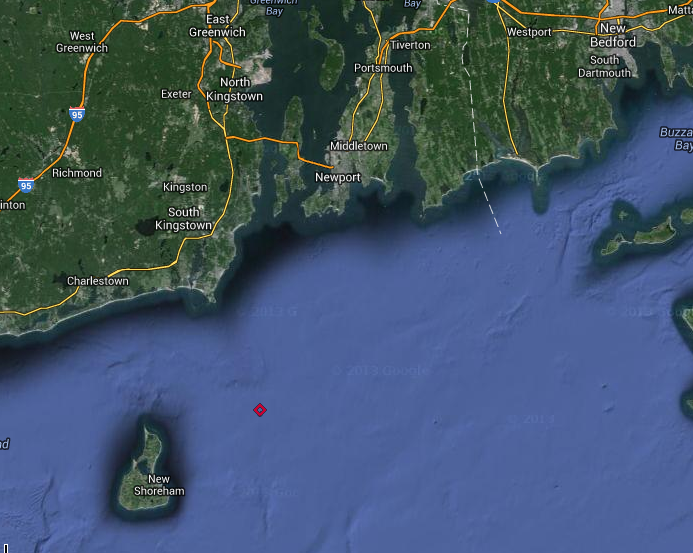
\includegraphics[width=0.7\textwidth]{./img/wislocation.png}
	\label{fig:wis1}
	\caption{Location of WIS station 63079}
\end{figure}

A collection of functions were provided for the purpose of this study in order to extrapolate information from this weather station. This included the $wavedir.m$ function which would extract the predominant wave directions from the hind-cast data. The $monthlyextrema.m$ function could be used according to these dominant directions in order to determine the maximum wave height per each month in a 20 year hind-cast interval. These maximums could be processed in using a Gumbel distribution in the $extremeDist2_new.m$.

A Gumbel distribution can be used in order to model the distribution of the maximums in a number of samples of various length. It can be used in order to model the distribution of maximum wave heights throughout a serious of sample periods. A Gumbel distribution can also be used in order to make predictions of certain wave heights occurring in the future.  

\section{Solution of the Problem}

20 years of hind-cast wave height data from the Rhode Island coastline was downloaded from the U.S. Army Core of Engineers Wave Information Studies (WIS) project. Due to the functions provided for this study being outdated, a parsing function was developed in order to convert the data from the WIS station in to a form which could be interpreted. This function would parse the date vector from the station data and arrange the array data in a way which interfaced with the provided functions.

Using the $wavedir.m$ function, a rose plot consisting of 30 degree intervals was generated which displayed the concentrations of wave direction present at the studied location. This rose can be seen in Figure 2.2.

\begin{figure}[H]
	\centering
	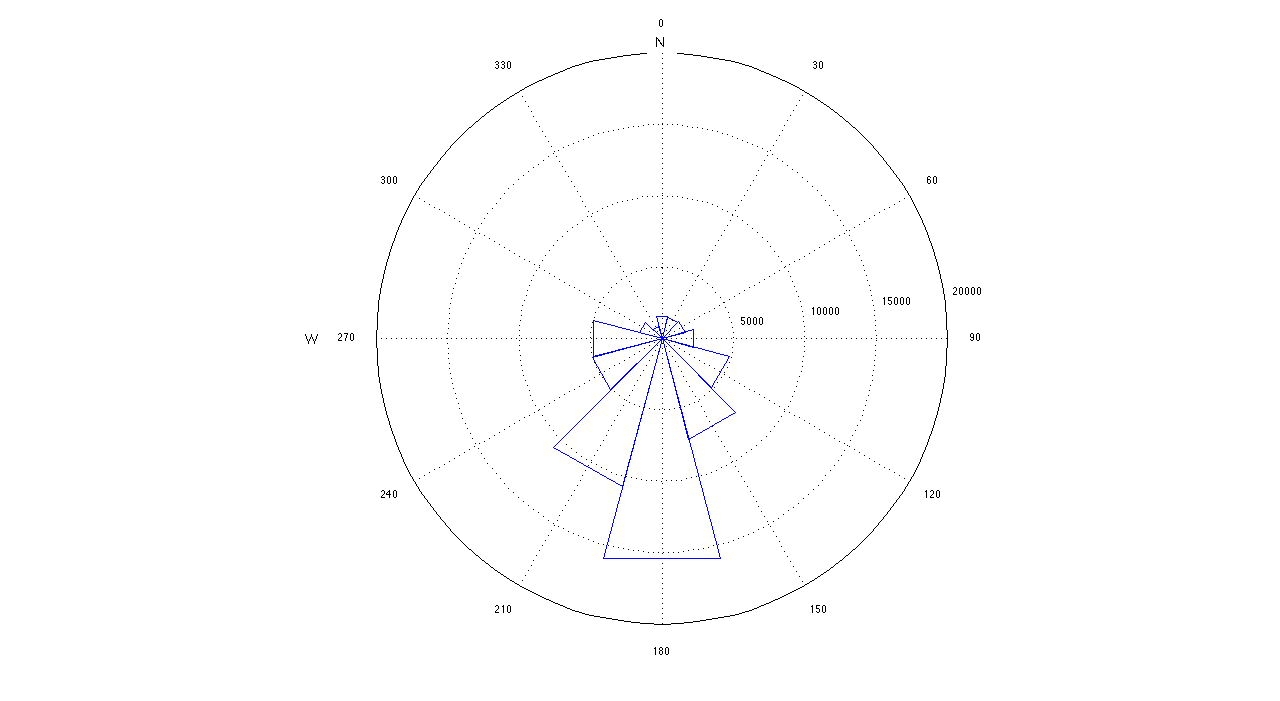
\includegraphics[width=0.7\textwidth]{./img/rose.png}
	\label{wisdir}
	\caption{Wave Directions at Station 63079}
\end{figure}

From this rose plot it can be seen that the predominate wave directions were 150$^{\circ}$, 180$^{\circ}$, and 210$^{\circ}$. The monthly maximums were then calculated for each of these three directions. This was done using the $monthlyExtrema\_new.m$, which would output the extrema data for each month to a text file for each direction. An example of this output can be seen in Appendix B.1. 

Using the $extremeDist2$\_$new.m$ function it was possible to render Gumbel distributions based off the calculated monthly extrema data. The distributions for angles 150$^{\circ}$, 180$^{\circ}$, and 210$^{\circ}$ respectively can be seen below in Figures~\ref{maxH150} through \ref{maxT210}.

\begin{figure}[H]
\centering
\begin{minipage}{0.49\textwidth}
	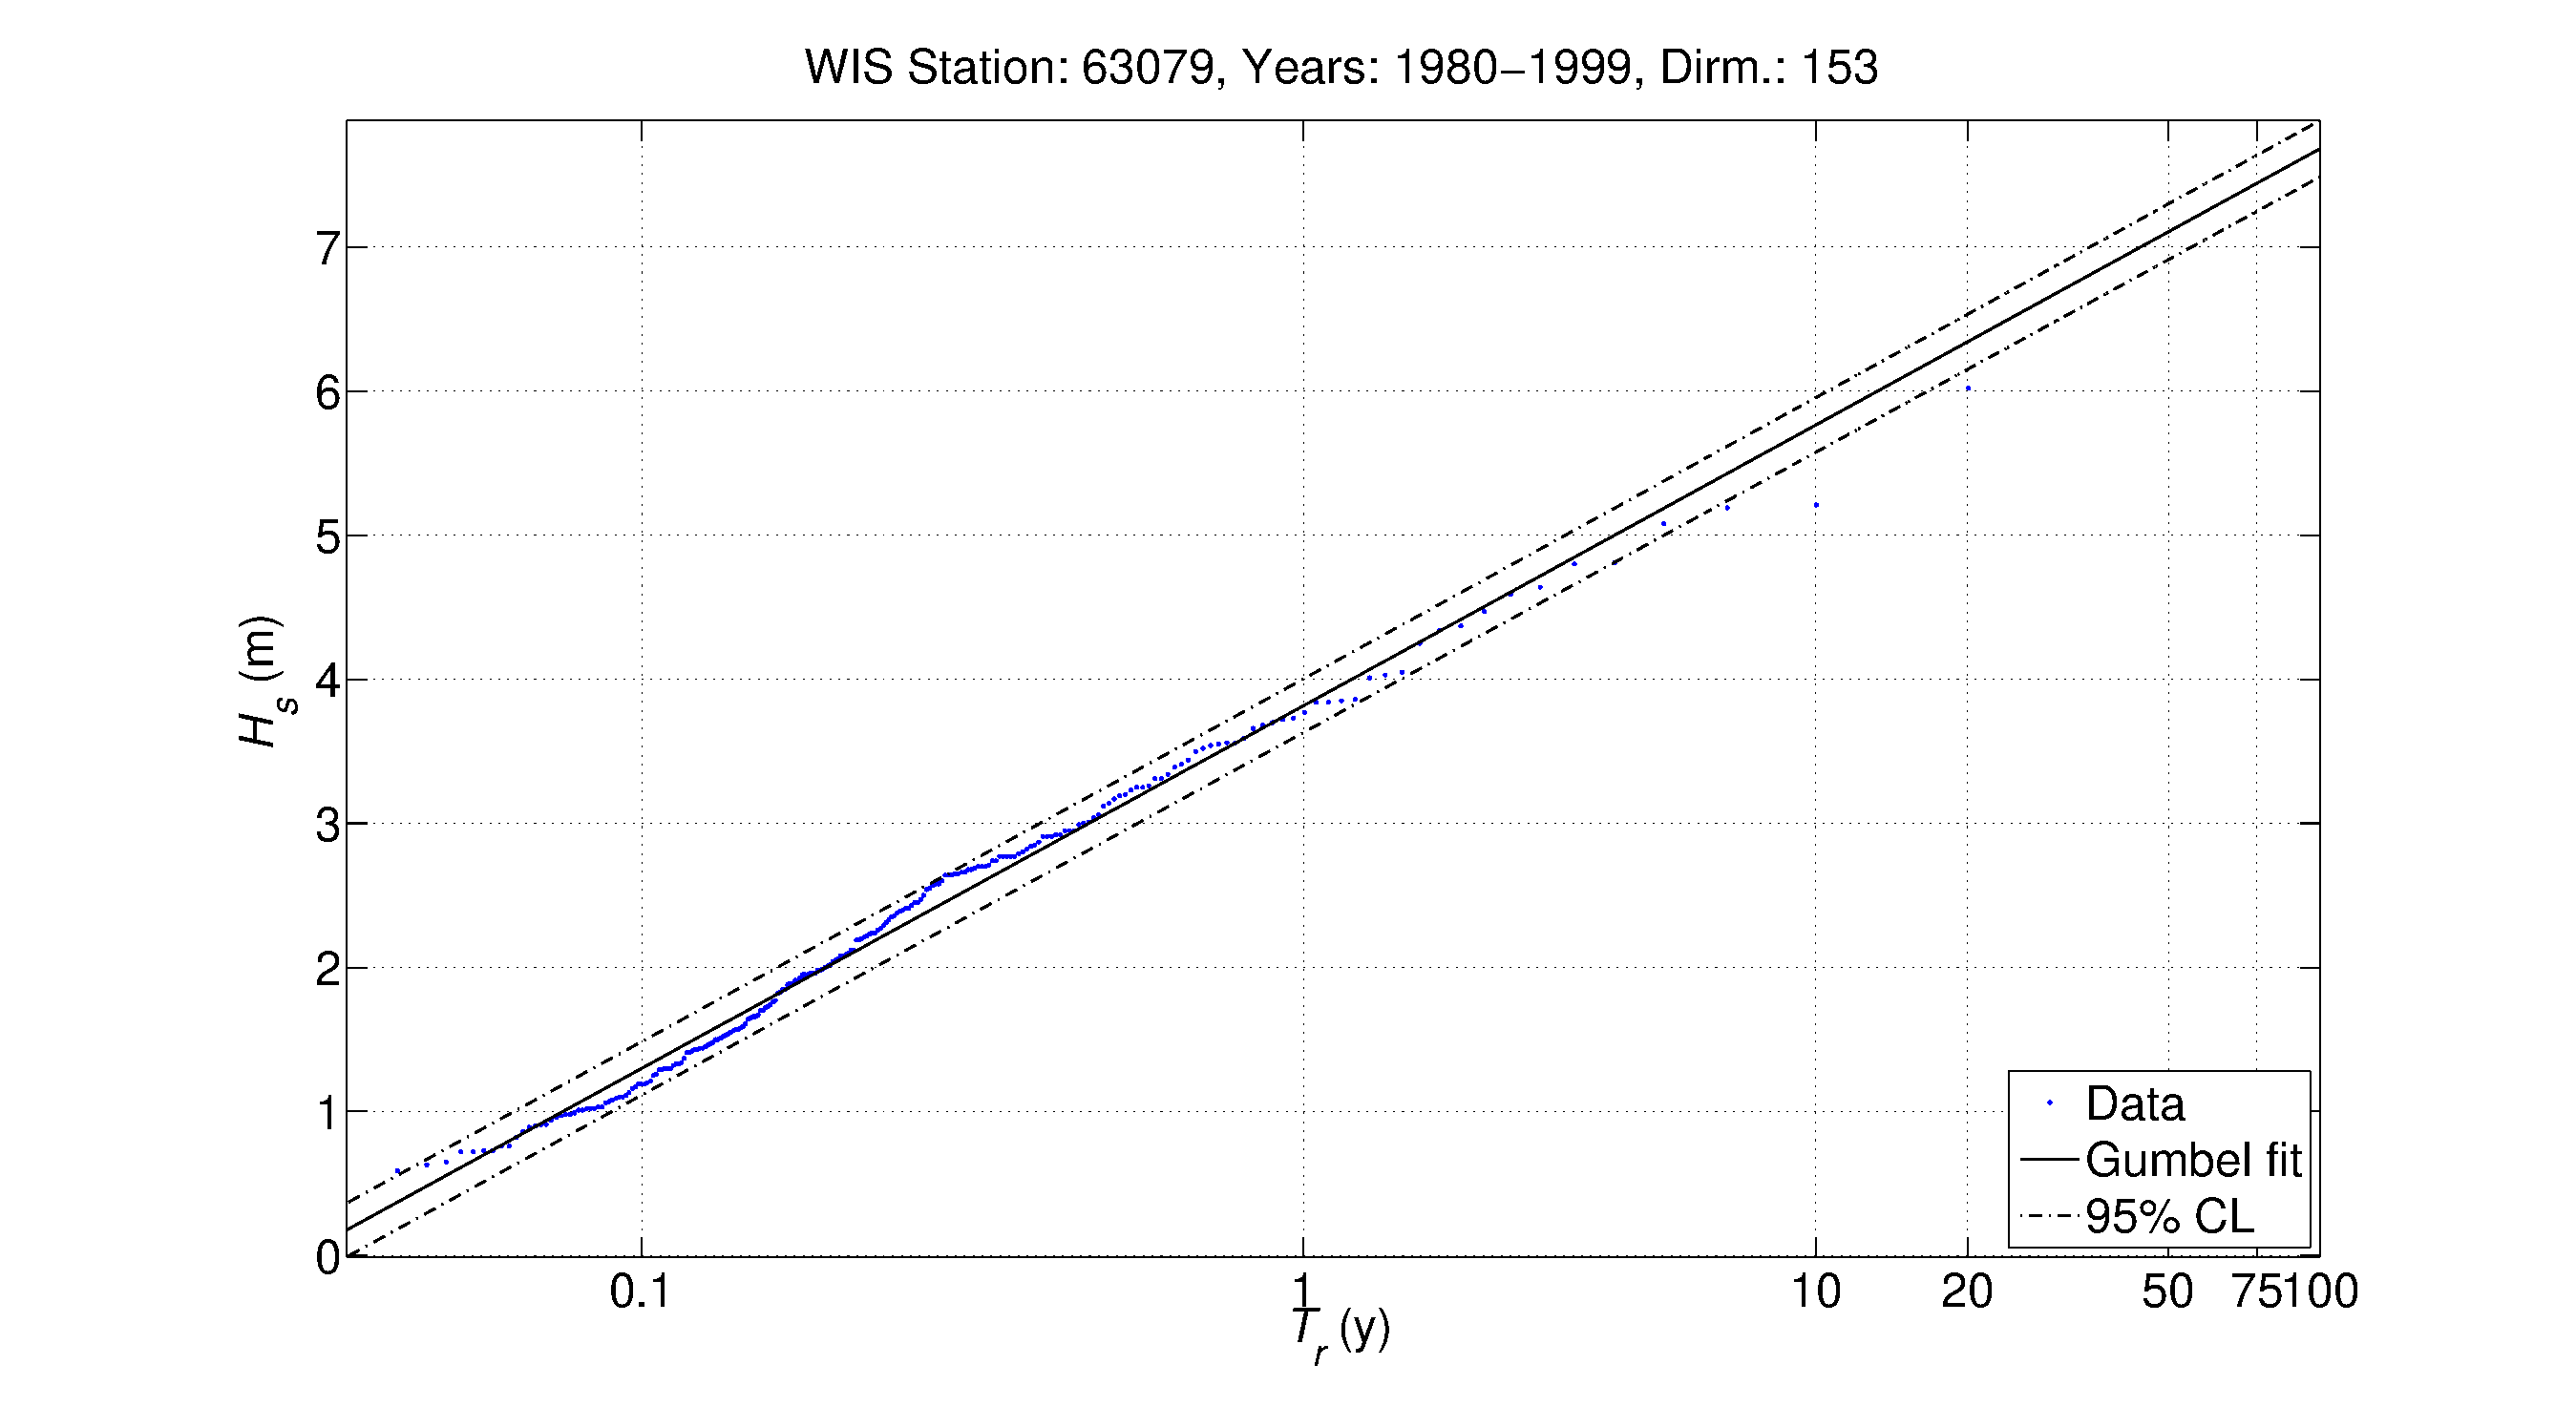
\includegraphics[width = \textwidth]{./img/150Hgumbel.eps}
	\caption{Gumbel distribution for Height at 150$^\circ$}
	\label{maxH150}
\end{minipage}
\begin{minipage}{0.49\textwidth}
	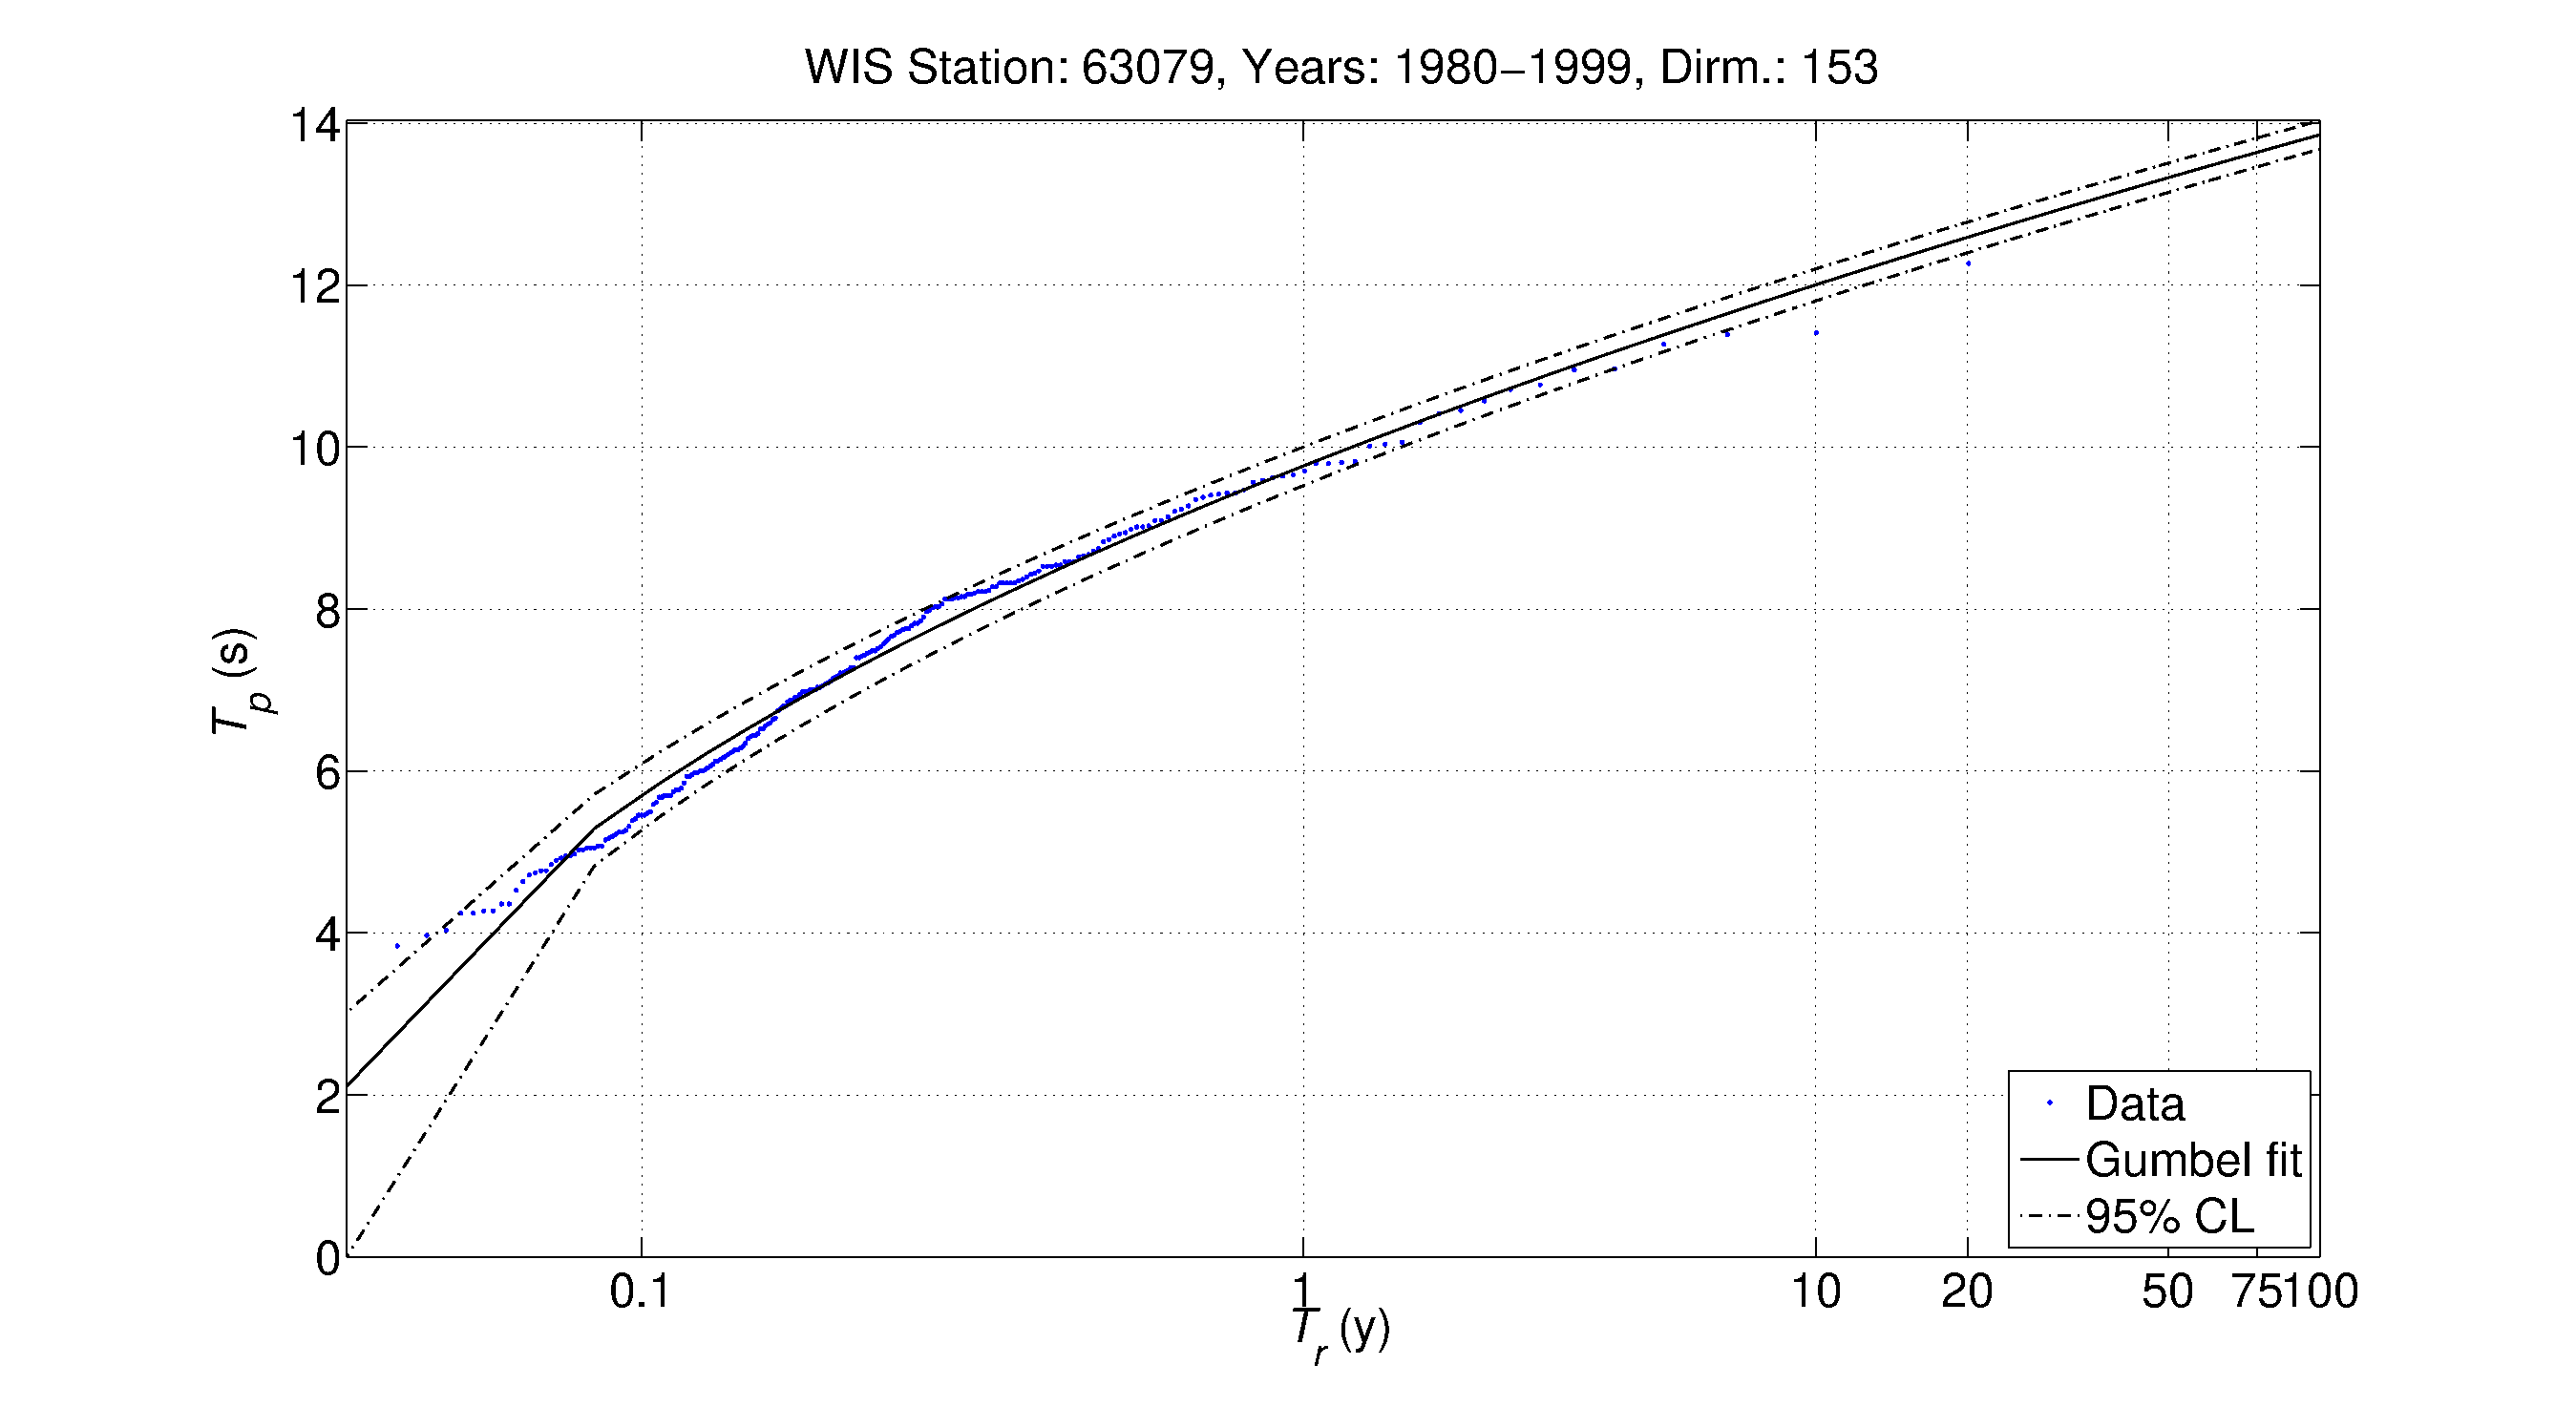
\includegraphics[width = \textwidth]{./img/150Tgumbel.eps}
	\caption{Gumbel distribution for Period at 150$^\circ$}
	\label{maxT150}
\end{minipage}
\end{figure}

\begin{figure}[H]
\centering
\begin{minipage}{0.49\textwidth}
	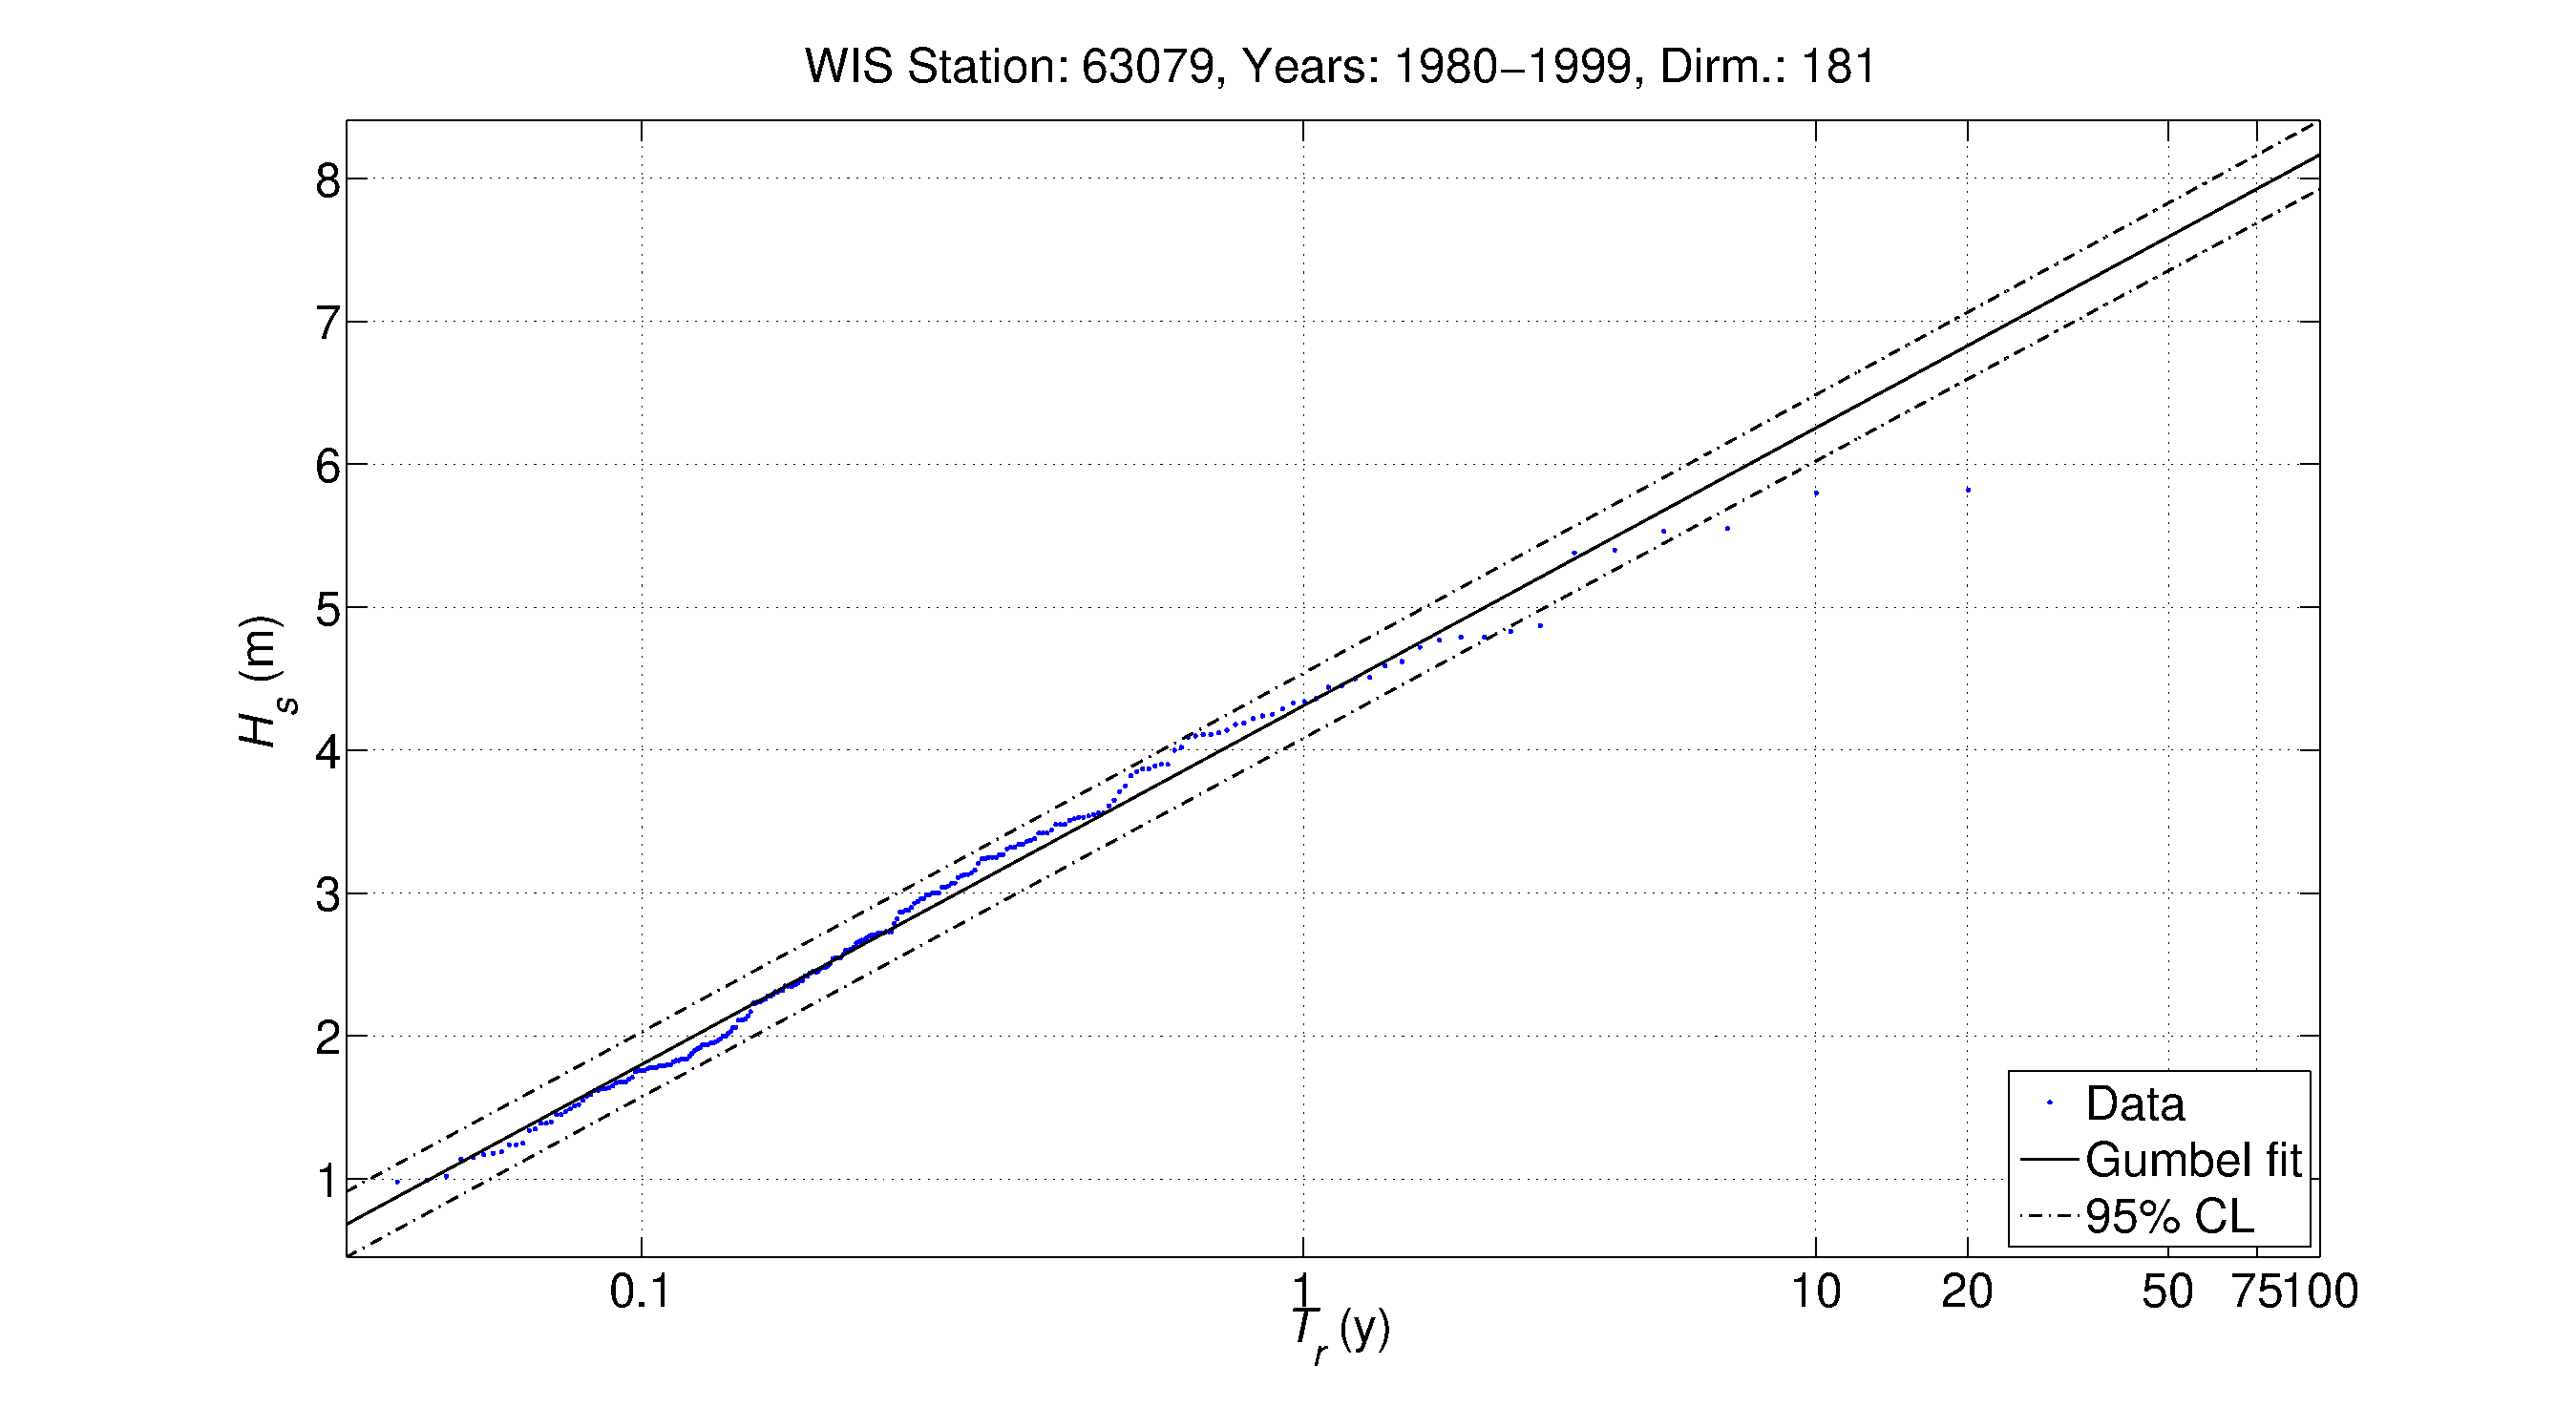
\includegraphics[width = \textwidth]{./img/180Hgumbel.eps}
	\caption{Gumbel distribution for Height at 180$^\circ$}
	\label{maxH180}
\end{minipage}
\begin{minipage}{0.49\textwidth}
	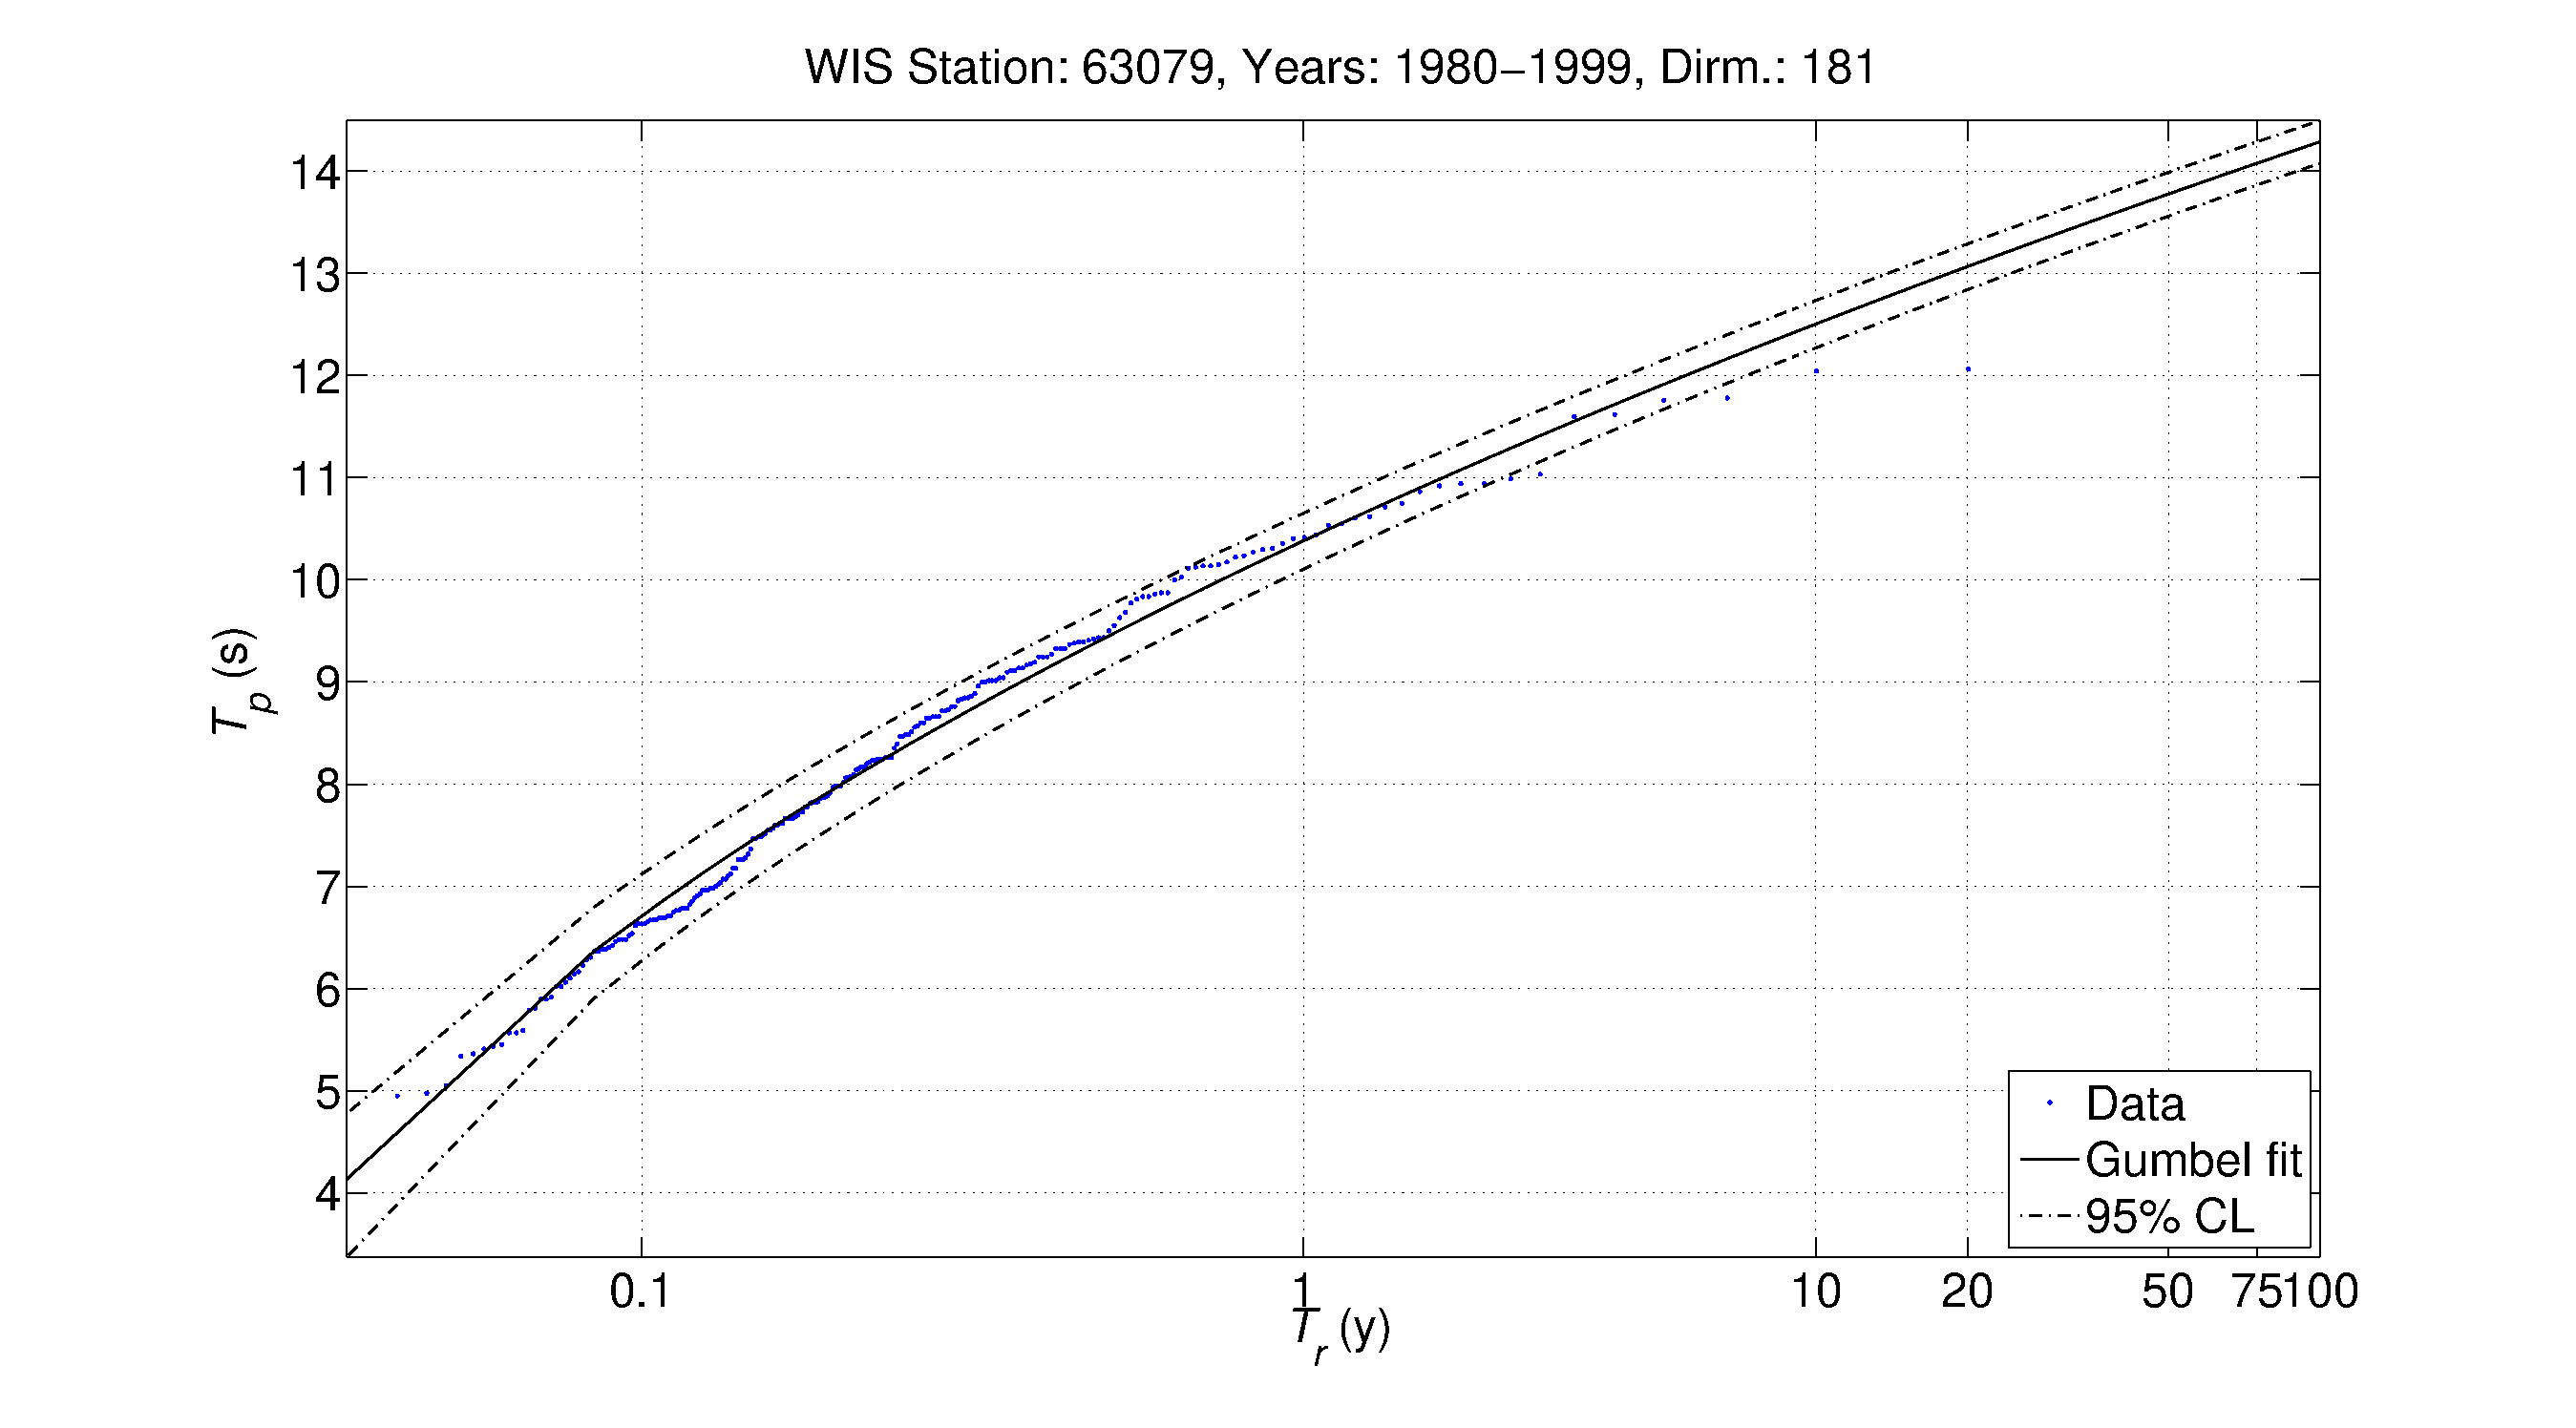
\includegraphics[width = \textwidth]{./img/180Tgumbel.eps}
	\caption{Gumbel distribution for Period at 180$^\circ$}
	\label{maxT180}
\end{minipage}
\end{figure}

\begin{figure}[H]
\centering
\begin{minipage}{0.49\textwidth}
	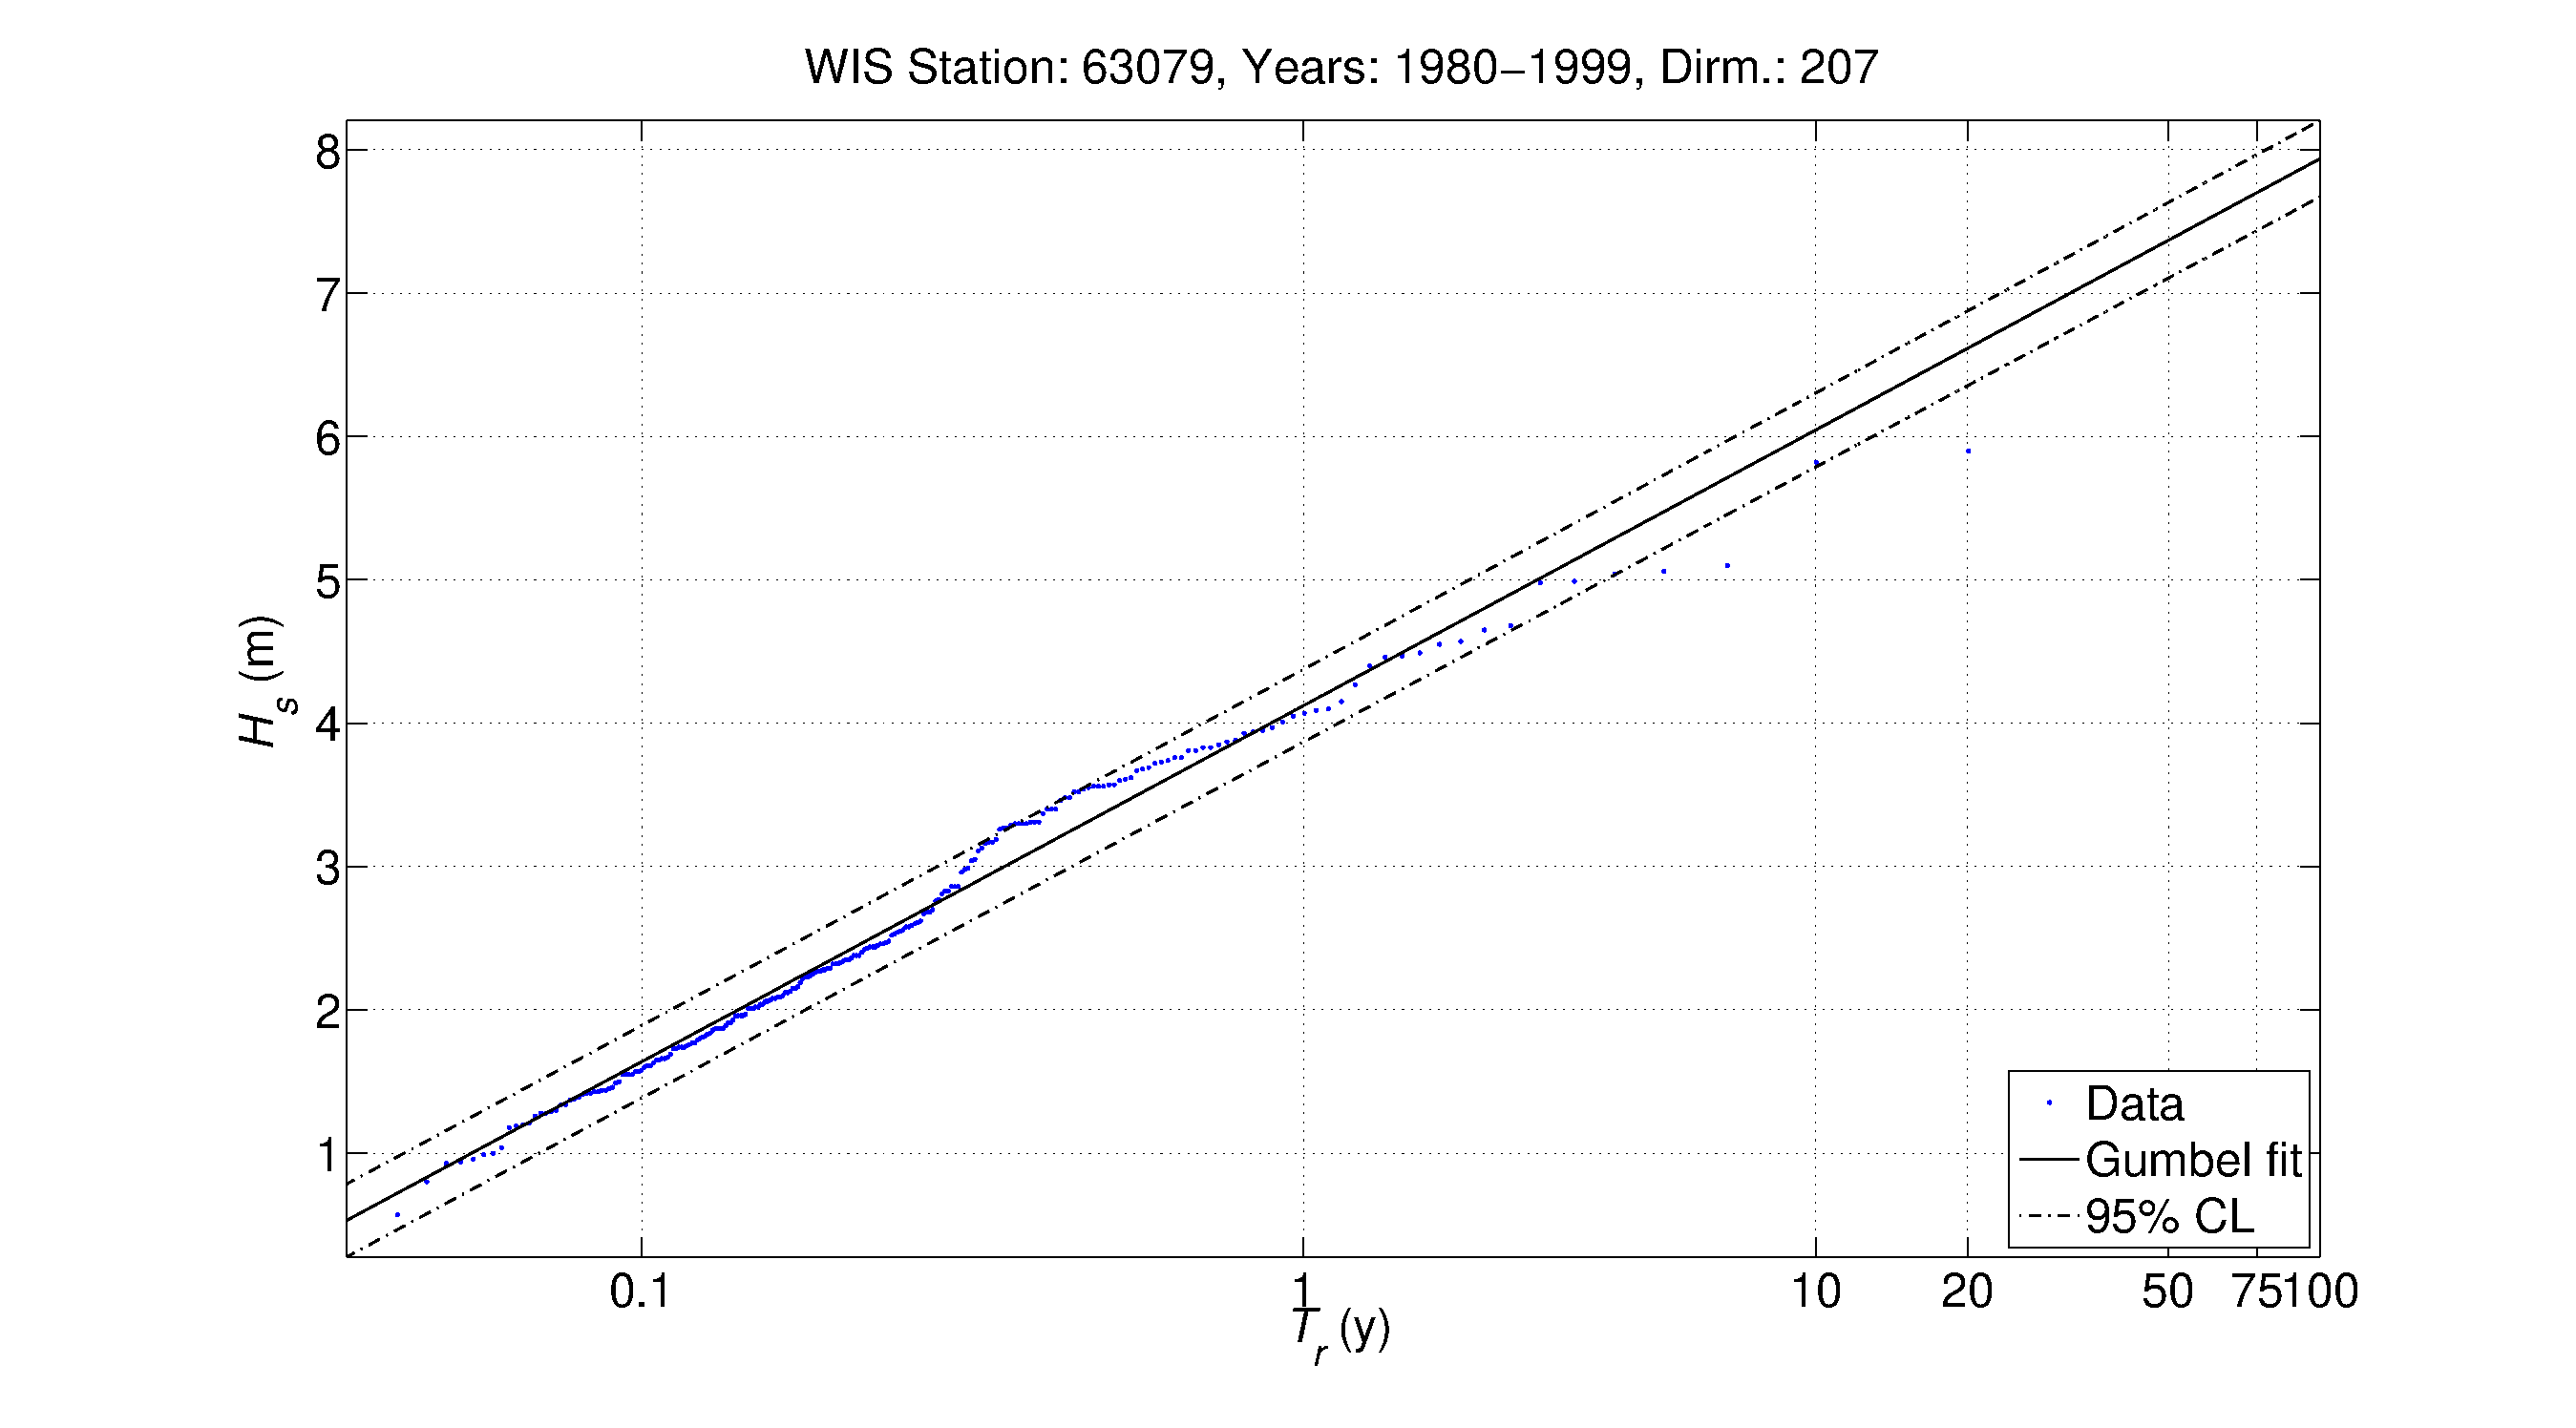
\includegraphics[width = \textwidth]{./img/210Hgumbel.eps}
	\caption{Gumbel distribution for Height at 210$^\circ$}
	\label{maxH210}
\end{minipage}
\begin{minipage}{0.49\textwidth}
	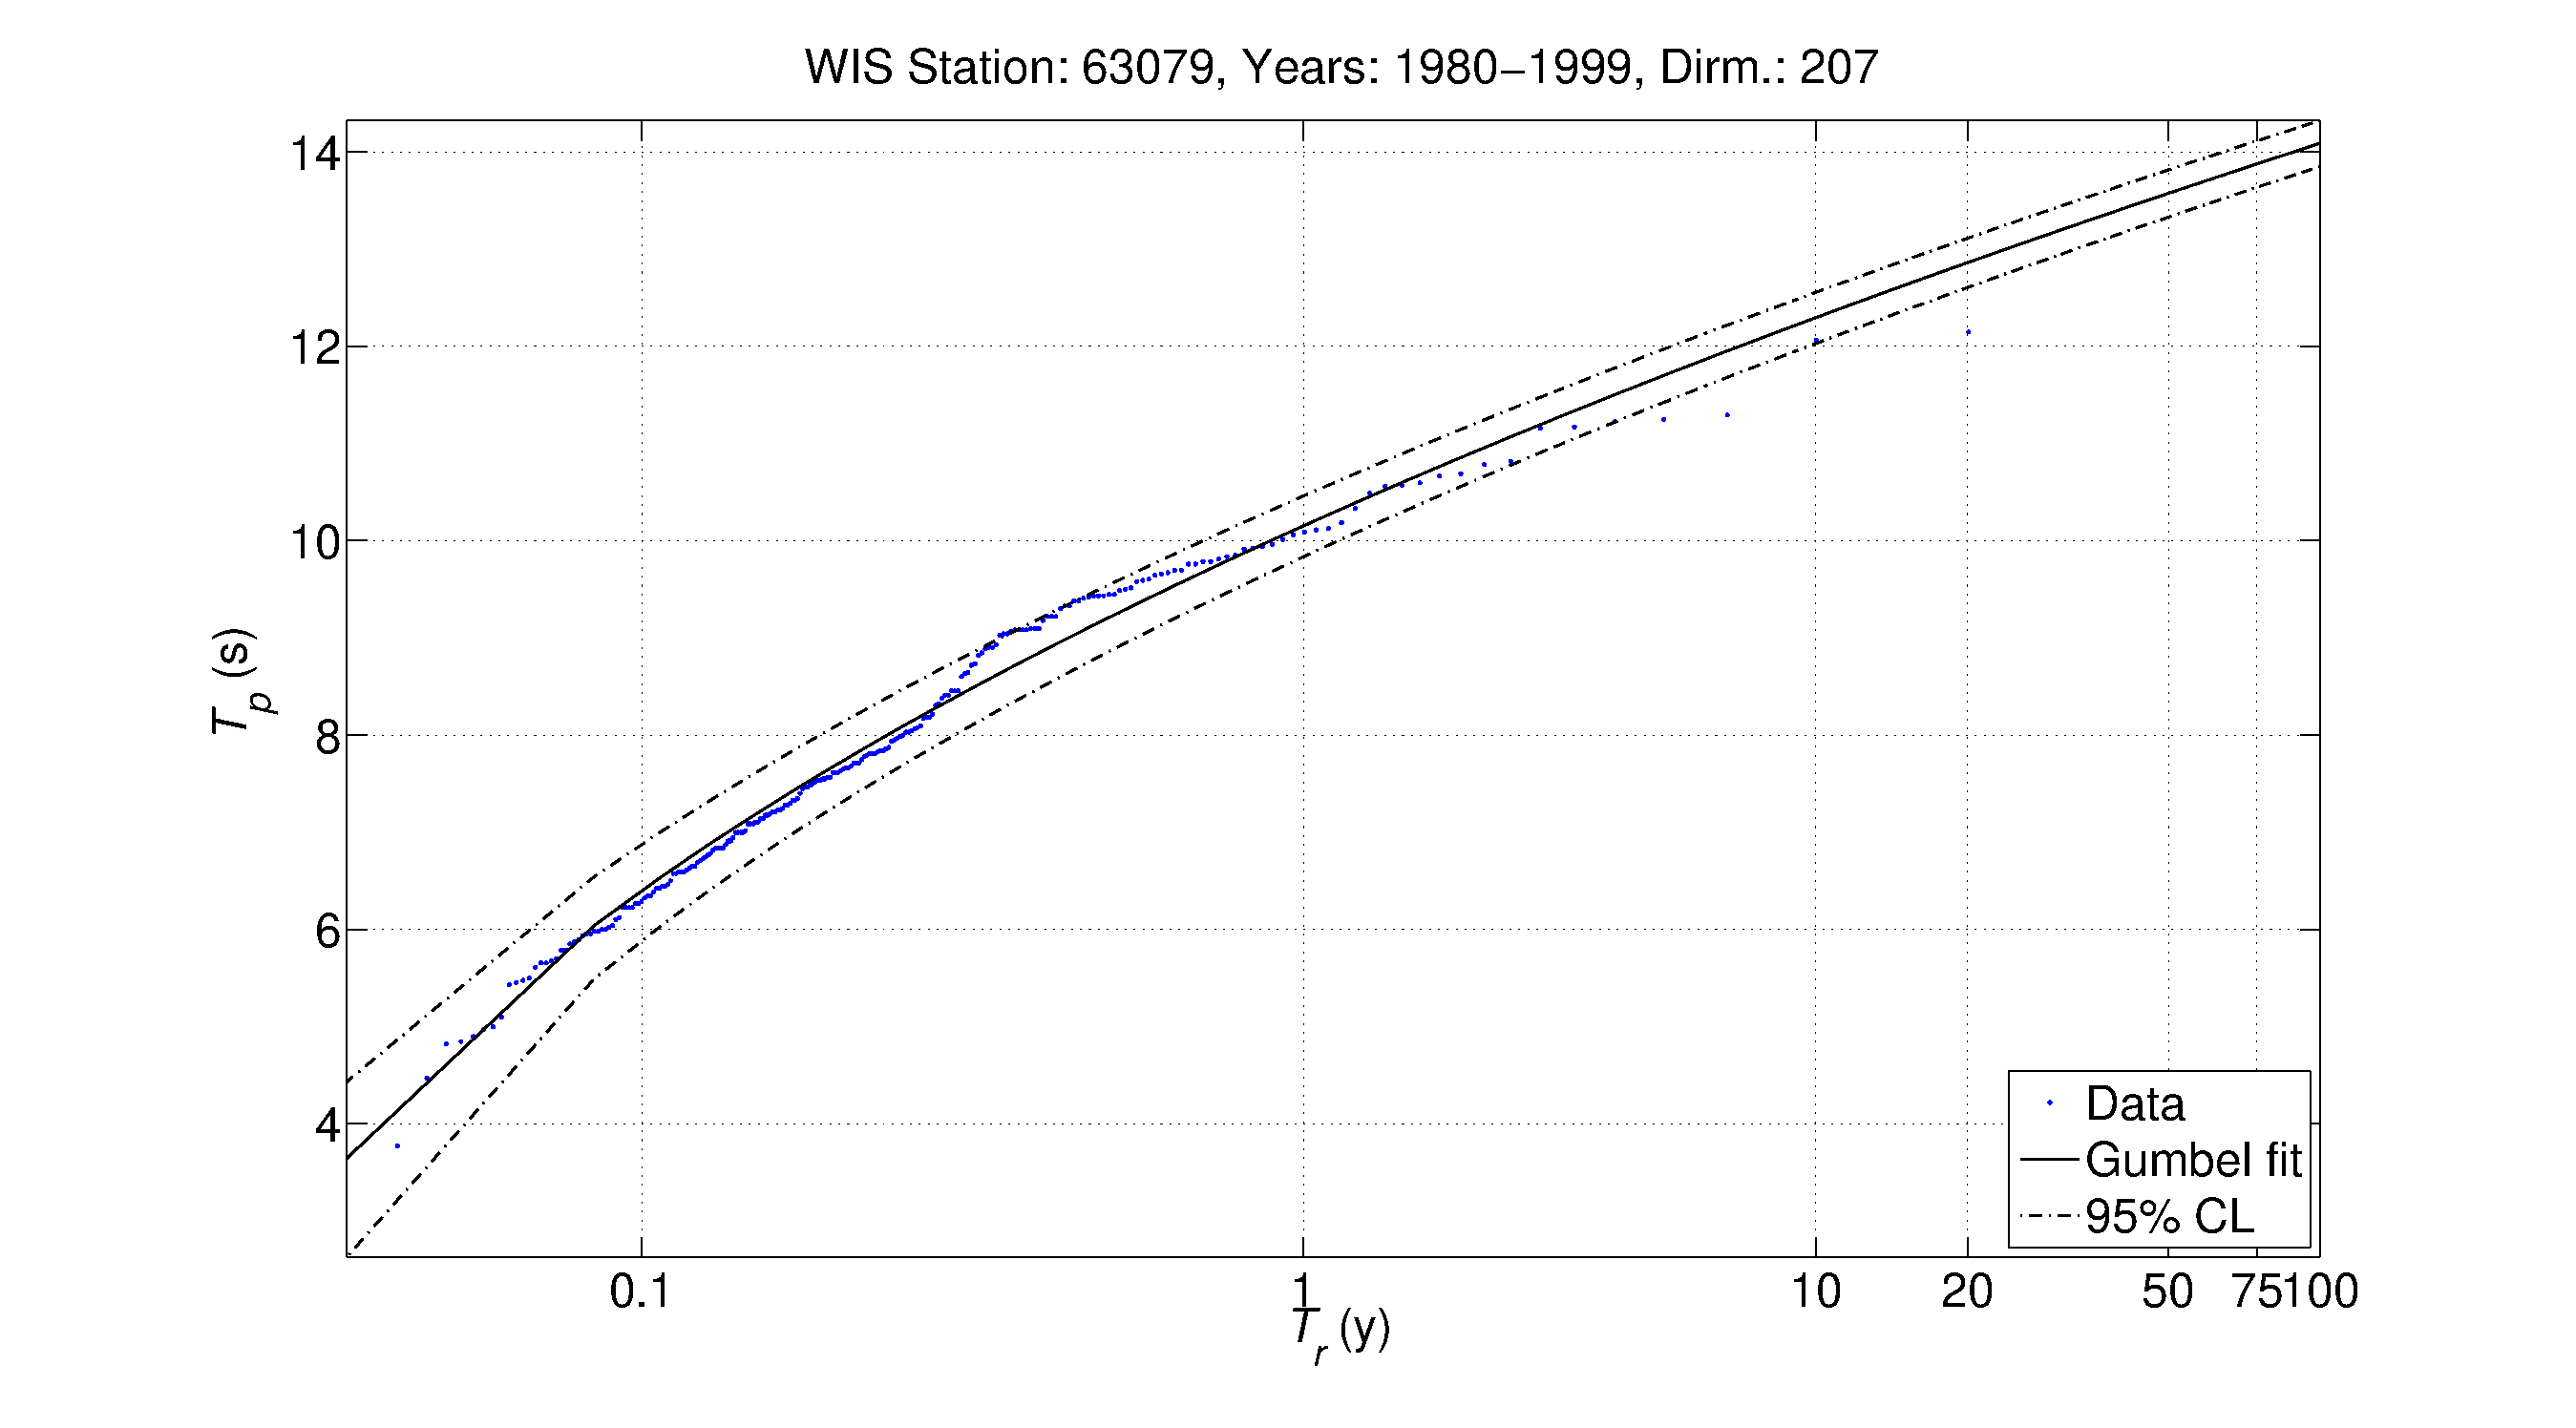
\includegraphics[width = \textwidth]{./img/210Tgumbel.eps}
	\caption{Gumbel distribution for Period at 210$^\circ$}
	\label{maxT210}
\end{minipage}
\end{figure}

The 20 - 100 year return parameters were also generated using the Gumbel distribution function. Tables containing this information for each dominant incident angle can be seen below in Tables~\ref{150T} through \ref{210T}.

\begin{table}[H]
	\centering
	\begin{tabular}{ccccc}
\hline
100.0 & 7.7 & 13.9 & 7.9 & 14.0 \\
75.0 & 7.4 & 13.6 & 7.6 & 13.8 \\
50.0 & 7.1 & 13.3 & 7.3 & 13.5 \\
20.0 & 6.3 & 12.6 & 6.5 & 12.8 \\
\hline
\end{tabular}

	\caption{150 degree return characteristics}
	\label{150T}
\end{table}

As can be seen in the above table, the function would compile maximum return characteristics for period intervals of 20, 50, 75, and 100 years. The function would return the maximum wave heights as well as the maximum periods. The following tables exhibited the same information for the other angles. 

\begin{table}[H]
	\centering
	\begin{tabular}{ccccc}
Tr (y)& Hs (m)& Tp (s)& CL95 Hs(m)& CL95 Tp (s) \\\hline
100.0 & 8.2 & 14.3 & 8.4 & 14.5 \\
75.0 & 7.9 & 14.1 & 8.2 & 14.3 \\
50.0 & 7.6 & 13.8 & 7.8 & 14.0 \\
20.0 & 6.8 & 13.1 & 7.1 & 13.3 \\
\hline
\end{tabular}

	\caption{180 degree return characteristics}
	\label{180T}
\end{table}

\begin{table}[H]
	\centering
	\begin{tabular}{ccccc}
Tr (y)& Hs (m)& Tp (s)& CL95 Hs(m)& CL95 Tp (s) \\\hline
100.0 & 7.9 & 14.1 & 8.2 & 14.3 \\
75.0 & 7.7 & 13.9 & 8.0 & 14.1 \\
50.0 & 7.4 & 13.6 & 7.6 & 13.8 \\
20.0 & 6.6 & 12.9 & 6.9 & 13.1 \\
\hline
\end{tabular}

	\caption{210 degree return characteristics}
	\label{210T}
\end{table}


\section{Conclusion}

The results from this task were used in order to generate projected wave rays towards Narragansett Town beach in Task 2. It was found that the dominant wave directions were accurately determined for later use. The resulting Gumbel distributions were also feasible. The data for the monthly extrema fit within the 90$\%$ confidence interval for the Gumbel for each direction. 
